%!TEX root = ../dissertation.tex
\begin{savequote}[75mm]
Eliminate all other factors, and the one which remains must be the truth.
\qauthor{-Sherlock Holmes, \textit{The Sign of Four}}
\end{savequote}

\chapter{Batch effect on covariance structure confounds gene coexpression}

\newthought{Systemic biases}
 associated with gene expression experiments, such as batch effects, have been known to induce spurious associations and  confound differential gene expression (DE) results. Commonly, to address the effects of batch on DE, methods have been developed to adjust expression values such that the mean and variance of each gene is conditionally independent of a set of batch covariates. To date, these methods have not addressed the potential for differential coexpression (DC) across confounders. While this is of lesser concern in the context of DE, analyses that utilize a gene coexpression or correlation matrix will continue to see confounding due to batch effects even when applying standard batch correction techniques. 

In this article, we demonstrate the persistence of confounding at the covariance level after standard batch correction using simulation and biological examples. We present an approach for computing a corrected gene coexpression matrix, called Coexpression Model Analysis (CMA), based on the estimation of a conditional covariance matrix. CMA estimates a reduced set of parameters that express the coexpression as a function of the sample covariates and can be used to control for continuous and categorical covariates. The method is computationally fast, and makes use of the inherently modular structure of features commonly found in genomic analyses.

\section{Introduction}

High-throughput data generation, including RNA-sequencing and microarrays,
have revolutionized molecular biology. These technological advancements
allow for the measurement of tens of thousands of gene expression
patterns at once, giving us a window into the molecular activity of
living cells. But as promising as these data generation methods are,
the deluge of data that has arisen from these tools has revealed an
extraordinarily level of complexity inherent to cells.  Muddying the links between the information detected at the gene level to the higher level observations of phenotypes.

Plummeting costs have lead to increased accessibility of high-throughput
genomic assays and with that we gain ability to investigate numerous
hypotheses simultaneously. At the heart of most genomic studies is
the analysis of the manner in which the biological variability of
genomic features, such as RNA expression, differs in the context of
phenotypes and/or other genomic features. We hope that understanding
the joint distribution of gene expression, conditional on phenotypes,
will lead to an understanding of the core biology. However, it can
be difficult to distinguish which associations are driven by real
biological mechanisms and which associations are observed because
of confounding by undesirable batch effects or other extraneous experimental
variables. It is critical to address this confounding in order to
reduce the probability of false positive results.

In the context of gene expression studies, the measurement of biological
sources of variation RNA abundance are typically of interest. Commonly,
observed variation is the result of technical artifacts that
may confound associations between experimental groups and gene expression
\cite{leek2010tackling,lander1999array}. 

Batch effects are known to come from many sources. Some sources are
obvious, such as the array platform or the experimental reagents used,
but others may be more unexpected. Timing, ozone\cite{fare2003effects},
technician and lab humidity have all been identified as sources of
unwanted variation and undoubtedly many other sources remain undiscovered\cite{scherer2009batch}.
In other words, variation attributed to batch is virtually unavoidable. Ideally,
experimental design will allow for single-batch experiments to be
performed, but studies may be too large for this to be practical.
Randomized batch assignment is recommended as an experimental design\cite{conesa2016survey},
but many investigations involve the use of publicly available data
(e.g. Gene Expression Omnibus, Genomics Data Commons) for which no
randomization is possible.

A common way to approach the batch correction problem is to consider
the model $G_{ij}=\alpha_{j}+X\beta_{j}+B\gamma_{ij}+\delta_{ij}\epsilon_{ij}$,
where $G_{ij}$ is the gene expression of gene $j$ for sample $i$,
$X$ is the design matrix, $\beta_{j}$ is a vector of regression
coefficients for gene $j$ for the columns of $X$. The next two terms
specify the additive and multiplicative impacts of batch. \textbf{$B$}
is an matrix of indicators for each of the batches, and $\gamma_{j}$
is a vector of additive batch effects on gene $j$. $\epsilon_{ij}$
is the error term and $\delta_{ij}$ is the multiplier of that error
term. Controlling for batch necessarily involves estimating the impact
of batch on the mean expression and the variance of that expression,
specifically $\gamma_{ij}$ and $\delta_{ij}$, for each gene. It
is generally not known what mechanism for batch effect is at fault
for a particular study and consequently, it is unknown which set of
genes and the magnitude of the effect on those genes. Therefore, without
knowing which features are susceptible to batch effect, it is typical
to estimate $\gamma_{ij}$ and $\delta_{ij}$ for each separately
gene in a study. 

Despite widespread literature published regarding the identification
and control of confounding due to batch effect \cite{chen2011removing,benito2004adjustment,leek2007capturing,johnson2007adjusting,nygaard2016methods},
batch effect correction has focused on adjusting for the effects of
batch on gene expression mean and variance at an individual level.
For example, ComBat \cite{johnson2007adjusting} uses an empirical
bayes approach to estimate the mean and variance parameters for each
gene and then computes an adjusted gene expression that controls for
these effects. Another approach, Surrogate Variable Analysis \cite{leek2007capturing},
uses a combination of measured covariates and singular value decomposition
to identify unknown sources of variation. These variables are estimated
and their effects regressed out of the gene expression matrix. These
approaches amount to a location-scale adjustment that is critical
for promoting the conditional independence of gene expression with batch. For
the purposes of differential gene expression analysis, this approach
is reasonably effective for both microarrays and RNA-seq data \cite{conesa2016survey}.

However, as our understanding of genomics grew, we recognized that
finding differentially expressed genes do not give a complete picture
of relationship between the transcriptome and phenotype. Cellular
states involve the complex combination of numerous biological processes
that are characterized by the behavior of large sets of interacting
genes. This understanding has lead to increased interest measuring
gene coexpression, the degree to which the expression between two
gene is correlated, to gain an understanding of the network biology
where simple differential gene expression falls short. Analogous to
differential expression and complementary to network inference, we
are interested in differential coexpression - the change
in gene correlation across experimental conditions \cite{fuller2007weighted}.

The difference between differential coexpression analysis and differential
expression is that we focus on the pairwise joint distribution of
genes as opposed to the marginal distribution of each gene. Essentially,
we assume that genes that are functionally related will exhibit a
correlated expression pattern across a set of experimental conditions
or samples - a "guilt by association" premise. Significant association between groups of genes may indicate a common functional
interaction. With this in mind, a natural goal is the identification
of those genes that are differentially correlated. Gene pairs or gene
sets that gain or lose their common expression pattern across experimental
conditions may implicate the biological pathways or functional mechanisms
that drive a particular phenotypic change.

Many methods have been proposed in for differential coexpression analysis,
most commonly in the context of gene network inference\cite{hsu2015functional}. Often, these
proposed algorithms start with the computation of correlation matrices
from the gene expression data\cite{tesson2010diffcoex,wgcna1,wgcna2,glass2013passing,southworth2009aging,choi2005differential,siska2017differential,yu2011link,amar2013dissection}.  
There is an assumption, often implicit, that the gene expression data
lacks heterogeneity or has heterogeneity sufficiently corrected. The
biases that persist in the coexpression matrix when homogeneity is
violated are rarely discussed or considered in the literature. Each
of the methods that use correlation matrices would benefit from estimated coexpression that has had the impact of batch effect reduced compared to
a Pearson correlation alone.

In estimating coexpression matrices, standard batch correction is
critical \cite{furlotte2011mixed}, but not sufficient. Location-scale
confounding on gene expression will reduce power and bias results.
This will inevitably lead to highly significant, but biologically
meaningless associations between large volumes of genes. Though the
common batch correction practices help mitigate this problem, they
fail to remove the impact of the type of batch effect that causes
differential coexpression patterns among genes in the absence of differential expression. Current methods treat
batch effect as acting on the marginal distribution of each gene and
ignore the possibility of changes to joint distributions. While some
impact on the joint distribution is addressed by removing the impact
of differential means and variances across batches it is insufficient
if the covariance itself is associated with batch. 

It is easy to conceive of scenarios where this phenomenon plays out.
For example, different experimental protocols across batches may induce
a coexpression difference by preferentially sampling cells with certain
active biological pathways for cell cycle or stress response. But
even simpler, batch effect for coexpression may be introduced merely
by differential biological variability. To illustrate this, recall
that correlation is roughly interpreted as the square root of the proportion
of total variability explained by true relationship between the genes (as opposed to other sources
of error and variance). Then two genes which are functionally related will only
be detected as such if there exists meaningful biological variability in both batches. For example, if the two genes are consistently in the same expression state across samples, their correlation will be near zero despite their interaction.  Greater variability in one batch compared to another will lead to differences in ability to capture coexpression. Subtle differences in protocol that lead to differences in
biological variability can not be removed with standard batch correction
methods.

The demonstration in Figure \ref{simulated_example} shows two examples
of uncorrected batch effect (left) impacting two genes in a study.
In the top row, batch effect alters the means and variances of the
two genes (location-scale model). In the bottom row, the means, variances
\emph{and} coexpression is impacted. Upon application of ComBat (Right)
to the uncorrelated genes, the two genes become independent as desired.
However, when applied to the conditionally coexpressed case (Bottom
row) we continue to observe differential coexpression across batches.

\begin{figure}
\includegraphics[width=1\columnwidth]{figures/simulated_example}\caption[Toy demonstration of impact of batch correction on coexpression]{In this toy example, we demonstrate which artifacts standard batch
correction is capable of correcting and which artifacts will remain.
In A-D, we show plots of two example genes before (left) and after
(right) correction, colored by their batch. In the top row (A,B),
we show a comparison of two genes which are conditionally independent
and demonstrate that location-scale batch correction appropriately
removes the marginal dependence between the genes. In the bottom row
(C,D), we show two genes that are conditionally coexpressed and illustrate
that batch correction may help mitigate the measured coexpression,
but the resulting coexpression is still a function of the batch membership.
Importantly, when comparing coexpression matrices, differing batch
proportions will bias the differential coexpression. In simulations
we demonstrate that in the absence of batched differential coexpression,
ComBat sufficiently controls the type I error. However, when coexpression
differs by batch, our false positive rate increases above the expectation
of the null model.}
\label{simulated_example}
\end{figure}

Though methods exist to consider the correlation of genes in the presence
of location-scale batch effect, no method exists that further allows
for the coexpression itself to be a function of batch. Similarly,
no method currently available returns a corrected coexpression matrix
rather than a corrected expression matrix.

While the impact of ignoring pairwise interactions may be negligible
for simple differential gene expression analyses, it is the differential coexpression patterns, rather than differential expression, that
are widely considered in the field of network inference\cite{de2010differential,chen2011removing,fukushima2013diffcorr}.
The impact of confounding due to differential coexpression in batches
remains critically unexamined.

In order to solve this problem, we need to create a model that describes
the coexpression matrix as a function of the experimental conditions
and batches. Classical regression models predict the expectation of
a response variable as a function of a set of predictors, but in coexpression analyses, we are interested
in the covariance. Some work has recently been published on the subject of modeling the covariance matrix\cite{hoff2012covariance,zou2016covariance},
but little has been studied in high dimensional or biological settings. 

Estimating the coexpression matrix faces at least two major challenges. The first problem
is that in the case of numerous batches or
continuous covariates, it may not be possible to estimate a coexpression
matrix using the sample covariance matrix form, $\frac{1}{n}\sum_{i=1}^{n}\left(X_{i}-\bar{X}\right)\left(X_{i}-\bar{X}\right)^{T}$,
where $X_{i}$ is the set of all gene expression values for sample
$i$. Another issue is that it requires the estimation of a very large number of parameters.
Given $p$ genes, there are $\binom{p}{2}$ pairwise correlations,
and each of these must be a function of the number of covariates.
For most high throughput gene expression studies where $N\ll p$,
we want to limit this parameter space in some way. Previous work has
shown the increased difficulty in reproducing coexpression across
studies\cite{schlauch2016estimating} likely owing to the high number
of parameters to estimate in noisy data. Recent work has allowed for
the imposition of sparsity on the gene covariance matrix \cite{bien2011sparse}
or precision matrix \cite{friedman2008sparse}, but the complexity
of biological systems make sparsity an unreasonable choice and computationally
burdensome to implement. 

In the method we describe here, CMA, we reduce the parameter
space by exploiting the modular nature of gene expression, estimating
only $N$ variables for each covariate, with each weight corresponding
to a eigenvector. This collects the information from many similarly
expressed genes by effectively borrowing information from similarly
patterned features. This allows us to estimate gene coexpression matrix
as a function of sample covariates. Our method is presented in a regression
framework that allows for the inclusion of continuous and categorical
covariates into the adjustment model.

\section{Methods}

\subsection{Approach}

In this manuscript we present a method for estimating the coexpression
matrix by modeling the matrix as a function of the largest components
of variation. Critical to our approach is the idea that although there
are $\binom{p}{2}$ pairwise gene-gene relationships, the true biology
can be predominantly explained by a much smaller set of variance components.
One way to identify these components is to compute the eigendecomposition
of the gene correlation matrix. We can then write the coexpression
matrix as a function of the experimental covariates and these eigenvectors.
Solving this formulation by minimizing the squared error will yield
a set of parameter estimates from which we can compute corrected coexpression
estimates.

\begin{figure}
\includegraphics[width=1\columnwidth]{figures/overview2}\caption[Workflow of CMA]{\textbf{Workflow of CMA}. CMA begins with a raw or normalized
gene expression dataset. (1) Standard batch correction (ComBat) is
applied to remove location-scale batch effect. (2) The overall coexpression
matrix is calculated. (3) An eigendecomposition of the overall coexpression
matrix is computed. The eigenvectors from this decomposition are then
used to re-estimate ``pseudo-eigenvalues'' that minimize the coexpression
error from the batch corrected expression data. (4) Fitted values
obtained from this estimation, in combination with the eigenvector
matrix, $\mathbf{Q}$, are used to estimated covariate-dependent coexpression
matrices such as for batch corrected network inference or differential
coexpression analysis.}
\end{figure}

Consider a set of $N$ samples with $q$ covariates measuring gene
expression across $p$ genes. Let $\textbf{x}_{i}=(x_{i1},\dots,x_{iq})^{T}$
denote the covariates for sample $i$ and let $\textbf{g}_{i}=(g_{i1},\dots,g_{ip})^T$
denote the gene expression values for sample $i$ for the $p$ genes.

In multivariate regression form we can express this as 
\[
\textbf{g}_{i}=\mathbf{\beta}^{T}\textbf{x}_{i}+\mathbf{\epsilon}_{i}\text{ for }i=1,\dots,N
\]
 where $\mathbf{\beta}$ is a $q\times p$ matrix of coefficients.

Equivalently,

\[
\textbf{G}=\mathbf{\beta}^T\textbf{X}+\mathbf{E}
\]

where $\textbf{G}$, $\textbf{X}$ and $\textbf{E}$ are each matrices
with column $i$ corresponding to $\textbf{g}_{i}$, $\mathbf{\epsilon}_{i}$ and $\mathbf{x}_{i}$, respectively.

Here, we make the usual multivariate assumption for $\textbf{E}$
that the rows $\mathbf{\epsilon}_{i},\dots,\mathbf{\epsilon}_{N}$
are conditionally independent, and follow distribution, $MVN_{p}(\mathbf{0}_{p},\Sigma_{i})$.
Notably in this paper, the covariance of $\mathbf{\epsilon}_{i}$
differ according to $i$.

Estimating the covariance structure for a set of $p$ genes typically
involves computing the sample covariance matrix, $S$, with entries
$s_{jk}=\frac{1}{N-1}\sum_{i=1}^{N}(G_{ij}-\bar{G_{\cdot j}})(G_{ik}-\bar{G_{\cdot k}})$.
However, as is typical in high-throughput settings, $p\gg N$, producing
an estimated covariance matrix $p\times p$ with column rank $\le N$.

To address this ``curse of dimensionality'',
numerous methods have been proposed. One might use a series of LASSO
regressions to estimate parameters in the inverse covariance matrix
\cite{meinshausen2006high}, or perform penalized maximum likelihood
estimation with the penalty on the inverse covariance matrix \cite{banerjee2008model,yuan2007model,friedman2008sparse}.
Each of these approaches imposes sparsity on the precision matrix,
effectively assuming a large degree of conditional independence between
genes. More recent work has explored imposing sparsity on the covariance
matrix itself, rather than the precision matrix \cite{bien2011sparse},
which allows us to assume widespread marginal independence of genes. 

The approach we take here involves estimating a covariance matrix
$\Sigma_{i}$ which depends on the batch and experimental design features
of sample $i$. An estimate of $\Sigma_{i}$ that allows all elements
of the matrix to vary freely can be obtained by separately estimating
the covariance matrix for each unique row of $\mathbf{X}$. However,
this approach in impractical for a large number of categorical covariates
or any continuous covariates. Additionally, it neglects the information
in other samples and other genes which can be used to gain a better
estimate of the coexpression. Given that groups of genes often behave
in distinct patterns, it is inefficient to estimate coexpression values
for every pairwise combination of genes.

Instead, we approach the problem by making use of the fact that genes
commonly behave in coexpressed modules, and that the dimensional space
is effectively much smaller than $p^{2}$. To do this, we decompose
the gene expression correlation matrix and find a set of eigenvectors
which explain the variation. We then attempt to infer a diagonal matrix
of ``pseudo-eigenvalues'', which minimize the square error. This
procedure allows us to reduce the parameter space from $p^{2}$ to
$p$ or less while still considering the bulk of the variability in
the data. Furthermore, in the application to the gene expression data,
the column rank of the coexpression matrix will be $N-1$, and the
number of non-zero eigenvalues will also be only $N-1$. Therefore,
we need only estimate the parameters corresponding to eigenvectors
with non-zero eigenvalues substantially reducing the parameter space
from $p$ to $N-1$.

Formally, for $\Sigma_{i}$ we estimate $\Sigma_{i}=\mathbf{Q}\mathbf{\Lambda}_{i}\mathbf{Q}^{T}$,
where $\mathbf{Q}$ is held constant as the set of eigenvectors from
the full coexpression matrix. In this formulation,$\mathbf{\Lambda}_{i}$
is a diagonal matrix with entries 
\begin{equation}
\mathbf{\Lambda}_{i,kk}=\mathbf{x}_{i}\mathbf{\Psi}_{\cdot k}\label{eq:Lambda_diag}
\end{equation}
 where $\mathbf{x}_{i}$ is the predictors for sample $i$ and$\mathbf{\Psi}$
is a $p\times q$ matrix of coefficients. 

Because we don't estimate the pseudo-eigenvalues after $k=N-1$, we
set $\mathbf{\Psi}_{\cdot k}=\text{\ensuremath{\mathbf{0}}}_{q}$
for all $k\ge N$. 

Intuitively, we can think of the parameter matrix $\mathbf{\Psi}$
as adjusting the eigenvalues as a function of the covariates to minimize
the coexpression error. It is straightforward to show that in the
case of a single batch and no experimental conditions, i.e. $\mathbf{x}_{i}=1$
for all $i\in N$, then$\mathbf{\Psi}$ becomes identical to the vector
of eigenvalues from the original covariance matrix.

\subsection{Likelihood function}

The likelihood function for a multivariate normal with mean $\mathbf{\mu}$
and variance-covariance $\Sigma$ is 
\[
\mathcal{L}\left(\mu,\Sigma\right)=\prod_{i=1}^{N}\frac{1}{\left(2\pi\right)^{\frac{p}{2}}|\Sigma_{i}|^{\frac{1}{2}}}e^{-\frac{1}{2}\left(\mathbf{G}_{i}-\mu\right)^{T}\Sigma_{i}^{-1}\left(\mathbf{G}_{i}-\mu\right)}
\]

The maximum likelihood estimation of $\mathbf{\mu}$ is simply the
vector $\mathbf{\bar{g}}=\frac{\sum_{i=1}^{N}\mathbf{g}_{i}}{N}$
and since $\mathbf{\mu}$ is independent of $\Sigma$ we can subtract
off the row means, yielding $\mathbf{G}_{i}^{*}=\mathbf{G}_{i}-\mathbf{\bar{g}}$.
And plugging in our index dependent covariance matrix from equation
\ref{eq:Lambda_diag} we have

\[
\mathcal{L}\left(\mathbf{\gamma}\right)=\prod_{i=1}^{N}\frac{1}{\left(2\pi\right)^{\frac{p}{2}}|\mathbf{Q}\text{diag}\left(\mathbf{x}_{i}\Psi\right)\mathbf{Q}^{T}|^{\frac{1}{2}}}e^{-\frac{1}{2}\left(\mathbf{G}_{i}^{*}\right)^{T}\left(\mathbf{Q}\text{diag}\left(\mathbf{x}_{i}\Psi\right)\mathbf{Q}^{T}\right)^{-1}\left(\mathbf{G}_{i}^{*}\right)}
\]
where $\text{diag}\left(\mathbf{x}_{i}\Psi\right)$ is defined as
a matrix with 0's in all off-diagonal entries and diagonal equal to
$\mathbf{x}_{i}\Psi$.

\subsection{Estimator}

In estimating the parameters in the matrix $\Psi$, we may consider
that each row, $i$, of $\Psi$ corresponds to the vector of contributions
from the $i^{th}$ eigenvector of $\mathbf{Q}$. With $\mathbf{Q}_{i}$
specifying the $i^{th}$ column of $\mathbf{Q}$ we have that $\mathbf{Q}_{i}^{T}\mathbf{Q}_{j}=0$
for all $i\ne j$ and $\mathbf{Q}_{i}^{T}\mathbf{Q}_{i}=1$ for all
$i,j\in1,2,\dots p$.

For some $h\in1,2,\dots p$, we seek to find the estimates $\hat{\Psi}_{h}$
which minimize the squared error of the estimated correlation matrices
defined as $\mathbf{G}_{i}\mathbf{G}_{i}^{T}$ for each sample $i\in1,2,\dots,N$.
By the Orthogonal Decomposition Theorem, the ``error residuals''
$\mathbf{Q}_{h}^{T}\left[\mathbf{G}_{i}\mathbf{G}_{i}^{T}-\mathbf{Q}_{h}\mathbf{X}_{i}\hat{\Psi}_{h}\mathbf{Q}_{h}^{T}\right]\mathbf{Q}_{h}$
will be minimized when they are orthogonal to the hyperplane spanned
by $\mathbf{X}$. Therefore, we can set the product below (Equation
\ref{eq:least_squares_zero}) equal to the zero vector to solve for
our estimator $\hat{\Psi}$.

\begin{align}
\mathbf{0}_{q} & =\sum_{i=1}^{N}\mathbf{X}_{i}^{T}\left[\mathbf{Q}_{h}^{T}\left[\mathbf{G}_{i}\mathbf{G}_{i}^{T}-\mathbf{Q}_{h}\mathbf{X}_{i}\hat{\Psi}_{h}\mathbf{Q}_{h}^{T}\right]\mathbf{Q}_{h}\right]\label{eq:least_squares_zero}\\
\mathbf{0}_{q} & =\sum_{i=1}^{N}\left[\mathbf{X}_{i}^{T}\mathbf{Q}_{h}^{T}\mathbf{G}_{i}\mathbf{G}_{i}^{T}\mathbf{Q}_{h}-\mathbf{X}_{i}^{T}\mathbf{Q}_{h}^{T}\mathbf{Q}_{h}\mathbf{X}_{i}\hat{\Psi}_{h}\mathbf{Q}_{h}^{T}\mathbf{Q}_{h}\right]\nonumber \\
\mathbf{0}_{q} & =\sum_{i=1}^{N}\left[\mathbf{X}_{i}^{T}\mathbf{Q}_{h}^{T}\mathbf{G}_{i}\mathbf{G}_{i}^{T}\mathbf{Q}_{h}-\mathbf{X}_{i}^{T}\mathbf{X}_{i}\hat{\Psi}_{h}\right]\nonumber \\
\sum_{i=1}^{N}\left[\mathbf{X}_{i}^{T}\mathbf{X}_{i}\right]\hat{\Psi}_{h} & =\sum_{i=1}^{N}\left[\mathbf{X}_{i}^{T}\mathbf{Q}_{h}^{T}\mathbf{G}_{i}\mathbf{G}_{i}^{T}\mathbf{Q}_{h}\right]\nonumber \\
\mathbf{X}^{T}\mathbf{X}\hat{\Psi}_{h} & =\sum_{i=1}^{N}\left[\mathbf{X}_{i}^{T}\mathbf{Q}_{h}^{T}\mathbf{G}_{i}\mathbf{G}_{i}^{T}\mathbf{Q}_{h}\right]\nonumber \\
\hat{\Psi}_{h} & =\left(\mathbf{X}^{T}\mathbf{X}\right)^{-1}\sum_{i=1}^{N}\left[\mathbf{X}_{i}^{T}\mathbf{Q}_{h}^{T}\mathbf{G}_{i}\mathbf{G}_{i}^{T}\mathbf{Q}_{h}\right]\label{eq:estimator}\\
\hat{\Psi} & =\left(\mathbf{X}^{T}\mathbf{X}\right)^{-1}\sum_{i=1}^{N}\left[\mathbf{X}_{i}^{T}\mathbf{Q}^{T}\mathbf{G}_{i}\mathbf{G}_{i}^{T}\mathbf{Q}\right]\nonumber 
\end{align}
Equation \ref{eq:estimator} provides an estimate for $\Psi_{h}$,
a $q$-vector specifying the contribution of eigenvector $h$ and
the $q$ covariates to the correlation structure in the $N$ samples.

The estimate $\hat{\Psi}$ represents the least squares estimate for
$\Psi$, which is equivalent to the maximum likelihood estimate under
normal error. Given the generous assumption of a properly specified
model, this estimate will be the most efficient estimator and will
asymptotically converge to the true parameter $\Psi$.

This provides a closed form solution to our problem. Given that the
computationally intensive steps involve matrix inversion, the computational
complexity is $\mathcal{O}(n^{3})$ or less, depending on the specific
implementation. This allows for relatively fast computation of corrected
coexpression matrix that is comparable to the simple Pearson correlation
computation, which has similar complexity. Using a computer with Intel(R)
Core(TM) i7-3630QM CPU @ 2.40GHz, and Microsoft R Open 3.2.5 linked
with multi-threaded BLAS/LAPACK libraries, the R implementation of
this method finished in 8.8 seconds on a dataset of 4000 genes, 400
samples and 2 covariates. 

\subsection{Corrected covariance matrix}

With the estimates obtained with our method, it is straightforward
to see how fitted values for the covariance matrix for each sample
or experimental condition can be obtained. Using the usual interpretations
of . Given an estimate for $\Psi$, $\hat{\Psi}$, we can now estimate
the batch-independent covariance structure as 
\begin{equation}
\hat{\mathbf{S}}=\mathbf{Q}diag\left(\bar{\mathbf{x}}\hat{\Psi}\right)\mathbf{Q}^{T}\text{ or }\hat{\mathbf{S}}=\sum_{i=1}^{p}\bar{\mathbf{x}}\hat{\Psi}_{i}\mathbf{Q}_{i}\mathbf{Q}_{i}^{T}\label{eq:corrected_coexpression}
\end{equation}
 where $\bar{\mathbf{x}}$ is a $q$-vector specifying the column
means of $\bar{\mathbf{x}}$,
\[
\bar{\mathbf{x}}=\frac{\sum_{i=1}^{N}\mathbf{x}_{i}}{N}
\]

The differential coexpression matrix between two conditions, defined
in binary as column 2 of $\mathbf{X}$, is computed
\begin{equation}
\hat{\mathbf{W}}=\mathbf{Q}diag\left(\mathbf{v}\hat{\Psi}\right)\mathbf{Q}^{T}\label{eq:parameter_interpretation}
\end{equation}
where $\mathbf{v}=\left(0,1,0,\dots0\right)_{q}$

\section{Results}

\subsection{Simulations demonstrate residual coexpression batch effect after
ComBat}

To illustrate the presence of batch effect in purportedly corrected
gene expression data, we performed an extremely simple simulation
to capture the effect. We simply took a gene expression dataset of
100 samples and selected 1000 genes at random to be in batch 1 and
labeled them \textit{New Gene 1, \dots, New Gene 1000}. We sampled
another set of 1000 genes and assigned them to batch 2, and added
that data to \textit{New Gene 1, \dots, New Gene 1000}. In essence,
for each ``simulated'' gene, there were 200 total expression observations
- 100 from one gene and 100 from a separate gene. Naturally, there
was substantial association with batch across the dataset. This is
seen in the highly significant differential expression across batches.
We also compared the differential coexpression across batches by plotting
the distribution of differential coexpression estimates between batch1
and batch 2. We compared this distribution to that of two randomly
assigned groups to show that the absolute differential coexpression
was much greater across batches.

We then applied ComBat to the data, removing the effect of the batch
assignment and performed the above assessments again. As expected,
the differentially expressed genes virtually disappeared. Interestingly,
the differential coexpression was only mildly reduced. Substantially
more gene-pairs were highly coexpressed across batch-groups than across
random-groups. This simple demonstration illustrates both the value
of ComBat in addressing location-scale batch effect and the need for
methods which address batch structure.

\begin{figure}
\textbf{A}\includegraphics[width=0.9\columnwidth]{figures/demo_diffexpress}

\textbf{B}\includegraphics[width=0.9\columnwidth]{figures/demo_diff_coex_density}
\caption[Simulations demonstrate batch correction on differential expression and coexpression]{\textbf{Simulations demonstrate batch correction on differential expression and coexpression.} The impact of ComBat on differential expression relative to differential
coexpression was evaluated using an illustrative example. A dataset
was generated for 1000 genes using real data, but with batch effect
induced via the replacement of half of each gene's expression values.
This rewiring created substantial differential expression and coexpression,
but only the differential expression was addressed completely with
ComBat, highlighting the need for additional methods to address this
problem.}

\label{demo_plots}

\end{figure}

\subsection{Improved coexpression estimates in \emph{In Silico} analysis}

We performed a simulation study to determine the relative performance
of our method in identifying differential coexpression in the presence
of coexpression batch effect. Gene expression for 400 samples were
simulated across 4,000 genes. The simulation study contained a balance
Cases/Control design with 200 samples per group. Similarly, ``Batch
A'' and ``Batch B'' were each assigned 200 samples. To generate
an unbalanced batch effect, 150/200 samples in Batch A were control
group samples, whereas 150/200 samples in Batch B were cases. 

Each gene was randomly assigned to one of 10 distinct modules, labeled
A-J. Modules A,B were labeled as background modules with the coexpression
pattern present in all samples, Module C was present in all Batch
A samples, Module D was present in all Batch B samples, Module E was
present in controls, Module F and G were present in cases. The coexpression
pattern of all other modules were present in no samples. Within each
module each gene was assigned a continuous value, $\gamma_{i}$, uniformly
random between $-a$ and $a$. For case-control modules, $a$ was
chosen to be $\sqrt{0.1}$ and for all other modules $a$ was set
at $\sqrt{0.2}$. The true coexpression between any two genes was
defined as $\rho_{i,j}=\gamma_{i}\gamma_{j}$. This yielded within
module correlation values in the range $\left(-0.1,0.1\right)$ for
cases/controls and $\left(-0.2,0.2\right)$ for batch and background
modules. The average absolute correlation between two case-control
coexpressed genes was $\rho=0.025$ with $R^{2}=0.000625$. The average
absolute correlation between two batch or background coexpressed genes
was $\rho=0.05$ with $R^{2}=0.0025$. 

The simulated study was run by generating 400 samples from a multivariate
normal distribution with 0-vector mean and covariance equal to the
correlation matrix described above for each sample.

The eigenvectors obtained demonstrate the tendency to isolate distinct
gene modules. Figure \ref{fig:Eigenvector_plots} shows this feature
along with the pseudo-eigenvalue contribution of each covariate. It
is important to note that the top eigenvectors do not necessarily
identify genes of interest in the case-control context. The estimate
$\hat{\Psi}$ is a $3\times p$ matrix with the first 20 columns plotted
in (Figure \ref{fig:Eigenvector_plots}B). The $i^{th}$ column and
$j^{th}$ row can be interpreted as the additional contribution of
the $i^{th}$ eigenvector for a 1 unit increase in the value of the
$j^{th}$ variable. This is analogous to standard regression, where
we can identify the estimated mean differences associated with a change
in a predictor. To identify differential coexpression for the $j^{th}$
variable, such as case-control, controlling for batch we need only
examine the values that deviate significantly from zero. The parameter
corresponding to the case-control variable successfully finds the
eigenvectors which best describe the genes differentially coexpressed
across cases/controls.

We evaluated the ability of CMA to capture case-control differential
coexpression relative to batch coexpression and background coexpression
(Figure \ref{fig:insilico_results}). For 4,000 genes there are 7,998,000
pairwise coexpression estimates of which 319,600 (4\%) are considered
case-control gene-pairs, and 159,600 (2\%) are considered batch.

\begin{figure}
\begin{center}
\includegraphics[width=1\columnwidth]{figures/EigenvectorPlots.png}
\end{center}\caption[Eigenvector plots showing separation of modular structure]{\textbf{Eigenvector plots show separation of modular structure.} CMA is designed to estimate sample specific
coexpression as a function of the sample covariates and the overall
coexpression eigenvectors. \textbf{(A)} Here we see the top six eigenvectors
plotted for all 4000 genes. Each point is colored according to that
gene's membership in a batch, case-control or background module. We
see that the eigenvectors tend to separate along with coexpression
modules. \textbf{(B)} Pseudo-eigenvalues for the top 20 eigenvectors
corresponding to the three covariates (intercept, batch, case-control).
Deviations from zero on the y-axis are indications of an unequal contribution
of the corresponding eigenvector to the fitted coexpression estimate.
Note that eigenvectors 5 and 6 have notable non-zero pseudo-eigenvalues
corresponding to case-control parameter.}
\label{fig:Eigenvector_plots}
\end{figure}


\begin{figure}
\begin{center}
\includegraphics[width=.45\columnwidth]{figures/NaiveDensity.png}
\includegraphics[width=.45\columnwidth]{figures/OursVsNaive.png}
\\
\includegraphics[width=.45\columnwidth]{figures/ourMethodDensity.png}
\includegraphics[width=.45\columnwidth]{figures/OursVsOthersROC.png}
\end{center}\caption[Comparison of methods for differential coexpression estimates]{\textbf{Comparison of methods for differential coexpression estimates in \emph{In Silico} data.} Fitted differential coexpression scores
for standard differential coexpression (upper left) vs CMA
(upper right) separated by true relationship. Pearson difference failed
to generate much power to predict true coexpression compared to background
and found batch effect at approximately the same rate as true effect.
CMA found true effects at vastly superior rates compared to
both background and batch effect. The predicted scores of non-background
genes for Pearson difference (x-axis) vs CMA (y-axis) demonstrate
improved ability to separate case-control effects (orange) from batch
effects (black). ROC curves show the relative performance in identifying
case-control genes compared to background genes (left) and batch genes
(right).}
\label{fig:insilico_results}
\end{figure}


\subsection{ComBat-corrected expression data still contains batch-associated
coexpression in ENCODE}

Above, we outline a theoretical basis for adjusting for differential
coexpression by batch. In short, we demonstrate how this particular
form of batch-effect could, in theory, lead to reduced power and biased
results. However, it remains to be seen whether this purported phenomenon
actually occurs in real gene expression datasets. One might hope that
the impact of batch on gene expression data occurs on each gene independently,
altering the distribution of expression within each batch. In that
scenario, existing approaches would be sufficient for removal of batch
effect and batch-associated differential coexpression would be virtually
absent. 

To demonstrate that differential coexpression by batch exists in the
wild, we selected publicly available data from the ENCODE project.
This dataset (GSE19480) contains 153 RNA-seq samples across 57820
ENSEMBL IDs from lymphoblastoid cell lines obtained from Yoruban HapMap
individuals. Reads were aligned using Bowtie \cite{langmead2009ultrafast},
and counts were produced using \emph{featureCounts }from the \emph{Subread}
program\cite{liao2014featurecounts}. Replicates were removed, yielding
samples from 63 individuals who were each sequenced at both the Yale
University and Argonne National Laboratory (126 samples in total).
Both centers used the Illumina Genome Analyzer II, which helps reduce,
but is known to not eliminate, batch effect. These two centers represent
the two batches to consider for correction. Since each batch contains
RNA-seq experiments on the same group of 63 individuals, one would
hope that in the absence of batch effect (or in the presence of satisfactory
batch correction) that there would be minimal differential expression
and coexpression between the batches.

We first ran LIMMA on the uncorrected data between Yale and Argonne
and observed 495 significant (FDR<.01) genes (Figure \ref{ENCODE}A).
We then applied ComBat to the data with Yale/Argonne as the batch.
ComBat uses an empirical bayes approach to make location/scale adjustments
for each gene, returning a gene expression matrix of corrected values.
We then reran LIMMA using the same Center partition and observed 43
(FDR<.01) significant genes. Unsurprisingly, this procedure removed
the differential expression across batches which is critical from
the removal of confounding effects in differential expression. 

Next we examined the distribution of differential coexpression between
the two batches (Figure \ref{ENCODE}B). We also generated null distributions
by randomly swapping the two centers for each of the 63 individuals
1000 times. Interestingly, despite the absence of differential expression
across batches, differential coexpression persists after batch correction.

\begin{figure}
\textbf{A}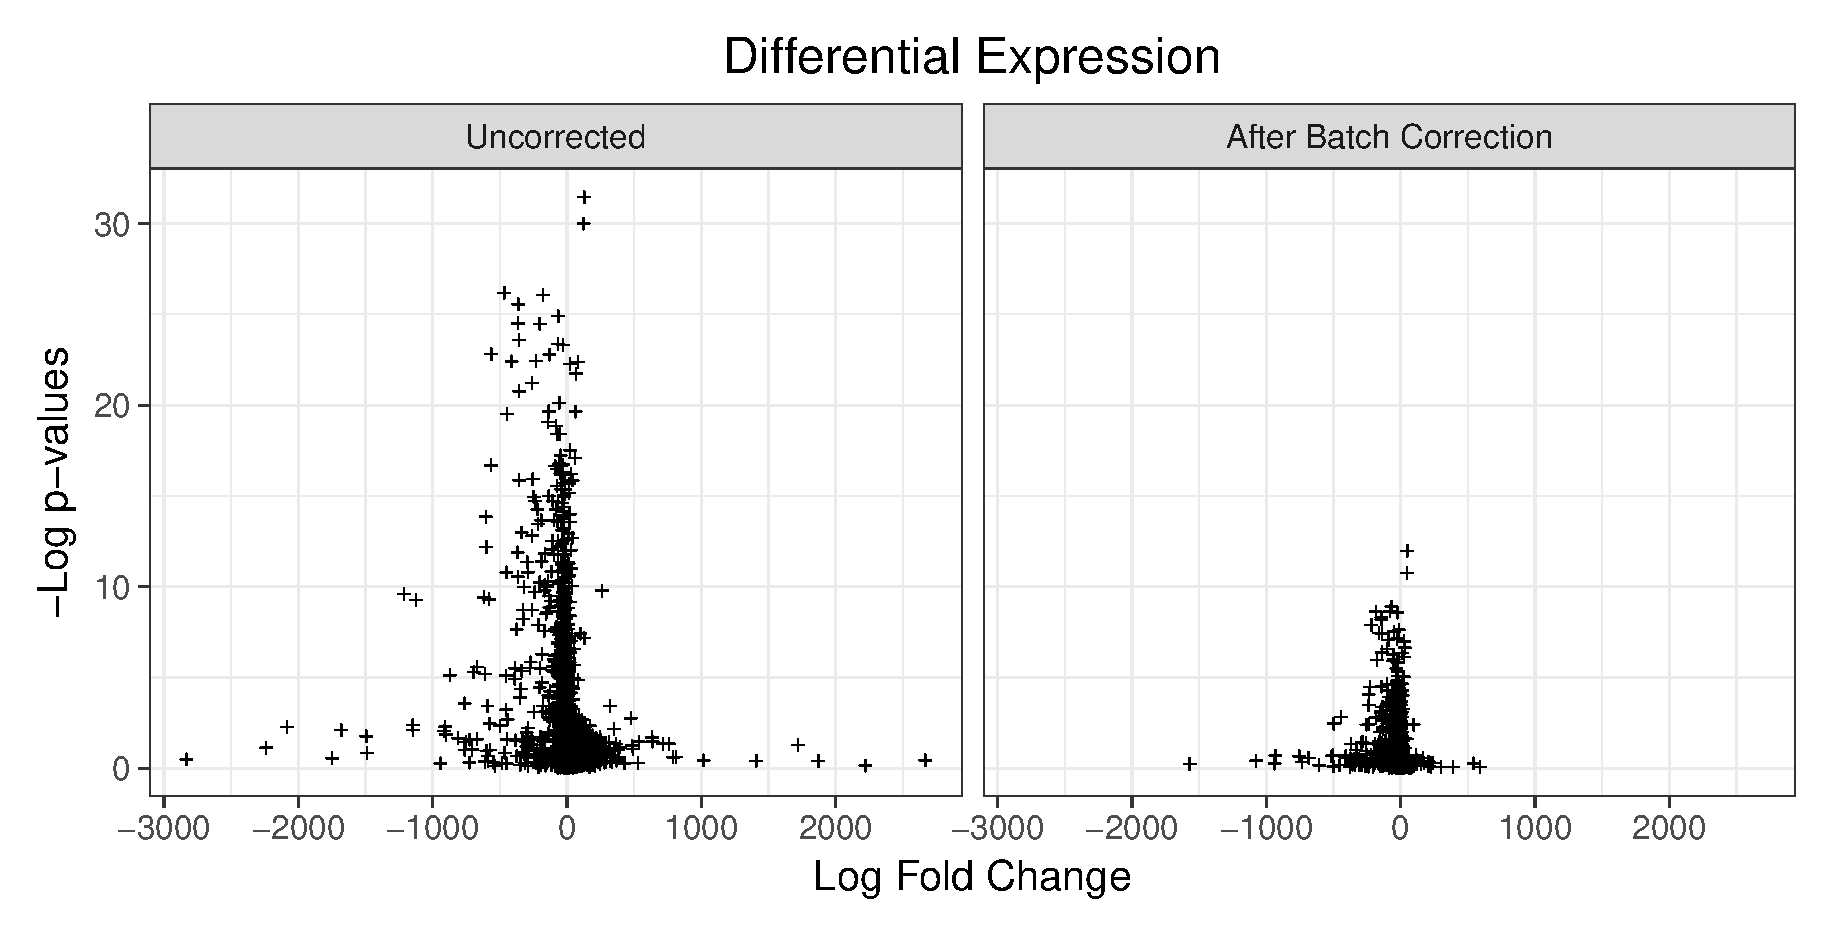
\includegraphics[width=1\columnwidth]{figures/encode_diffexpress}\\
\textbf{B}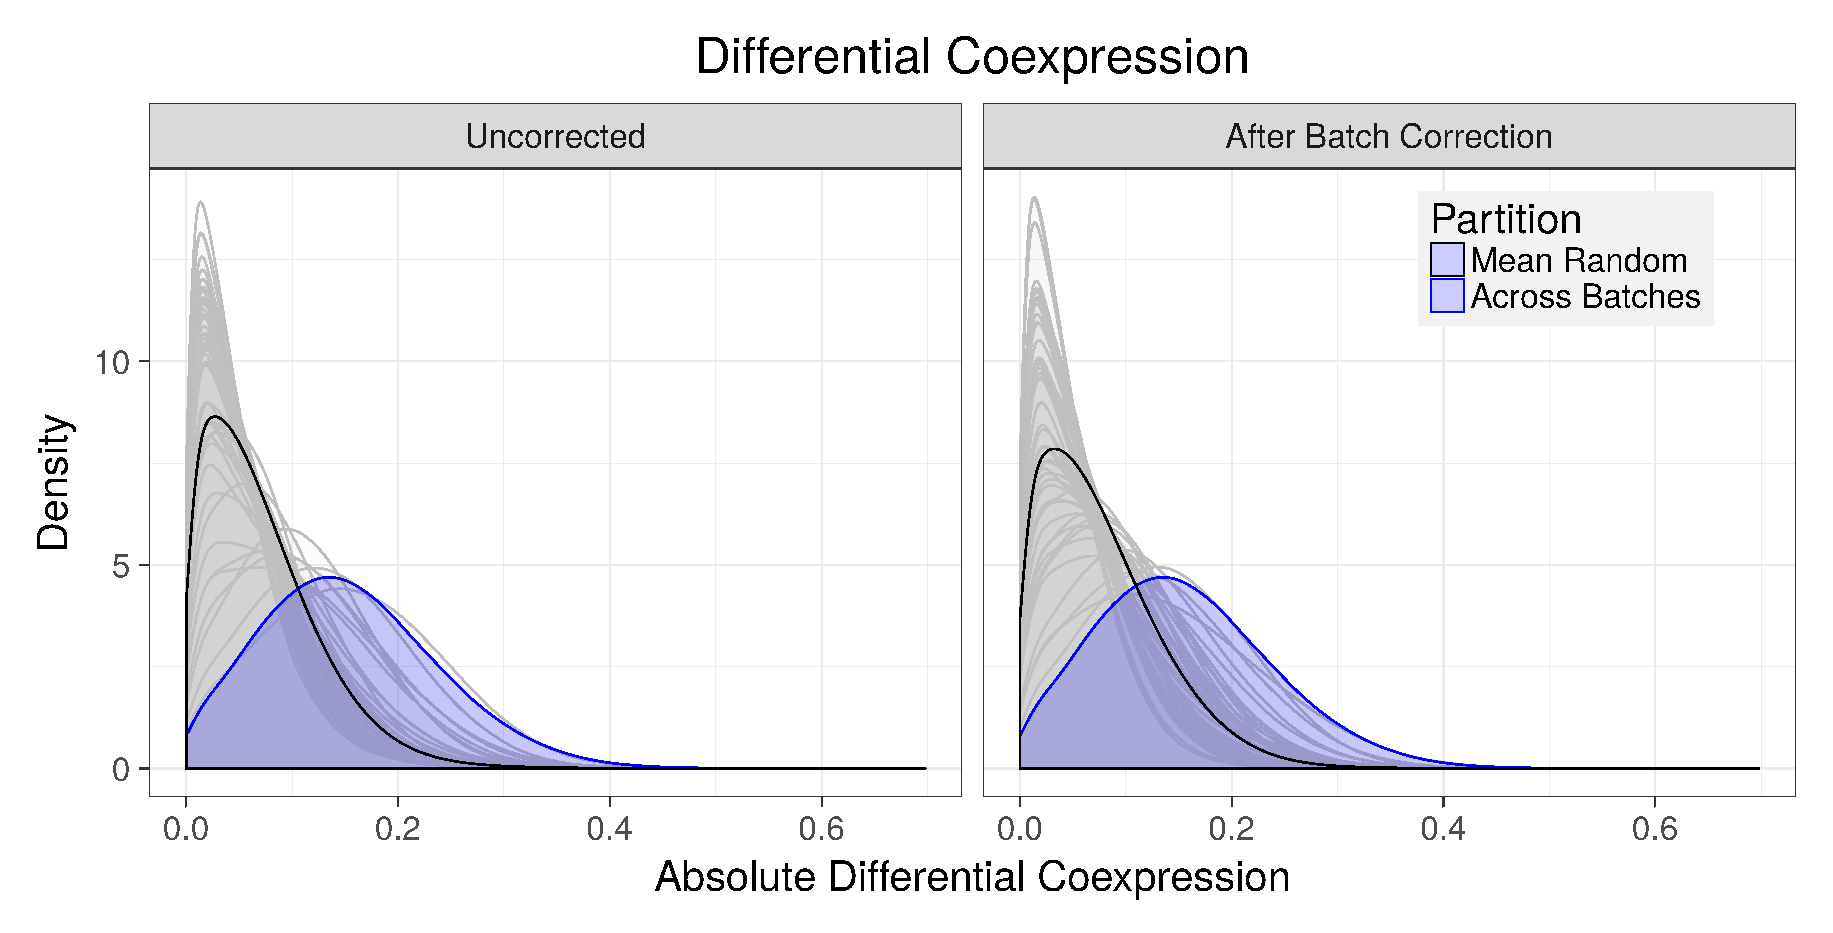
\includegraphics[width=1\columnwidth]{figures/encode_diff_coex_density}\caption[Differential expression and absolute differential coexpression in
ENCODE data with batch correction]{\textbf{Differential expression and absolute differential coexpression in
ENCODE data with batch correction}. ComBat effectively mitigates the
differential expression between samples run in two separate centers
(\textbf{A}). However, with this same batch correction, differential
coexpression continues to be strongly influenced by processing center.
The lower plot (\textbf{B}) shows the distribution of differential
coexpression when comparing groups that are randomly assigned (grey)
compared to assignments based on batch. Despite the fact that ComBat
helps mitigate differential expression between batches, these results
show that batch-associated differential coexpression remains uncorrected.}
\label{ENCODE}
\end{figure}


\subsection{CMA allows for separation of covariate specific modules with
WGCNA in COPDGene study}

Weighted Gene Coexpression Network Analysis (WGCNA) is one of the
most popular network reconstruction methods in use today \cite{wgcna1},
with 1730 citations as of March 31, 2017. Its use continues to grow
with 140 citations in the first 3 months of 2017. Like many other
methods in the field, WGCNA begins with a standard Pearson correlation
matrix of gene expression data. We were interested in whether the
use of CMA could provide covariate-specific differential coexpression
estimates that could integrate with WGCNA to find functionally relevant
coexpression modules. While our method is motivated by the idea of
removing batch, it is general enough to be applied to any confounding
variable. In this application, we chose to treat three clinical covariates as confounders - sex, age and pack-years. 

Gene expression data from the COPDGene study (GSE42057)~\cite{bahr2013peripheral,regan2011genetic}
was collected from blood samples obtained from 136 subjects classified as smoker controls (42) or COPD (94) and profiled on  Affymetrix Human Genome U133 Plus 2.0  microarrays. CEL data files from these microarray assays were RMA-normalized using the 'affy' package and array probes were collapsed to Entrez-gene IDs using a custom CDF\cite{dai2005evolving}, yielding 18,960 genes.

Previous work applying WGCNA to this data has identified network modules
associated with COPD diagnosis\cite{morrow2015identifying,morrow2017functional}.
These studies involved applying topological overlap to an overall
similarity score (e.g. Pearson, Euclidean, biweight midcorrelation)
after standard batch correction (Surrogate Variable Analysis\cite{leek2007capturing}).
The similarity matrix typically does not consider sample covariates
and consequently yields a collection of modules which are generally
coexpressed, not necessarily differentially coexpressed. To identify
which modules might be relevant to phenotypes of interest, an eigendecomposition
by samples of each module is performed and the top eigenvector (eigengene)
is regressed against the phenotypes and other covariates. This approach,
while effective at identifying associated modules has limitations.
The eigengene obtained through this method will capture the greatest
axis of variation across the samples, not the greatest axis of covariation.
By design, the eigengene will only be associated with a phenotype
of interest if there is differential expression within the module
across phenotypes. Given the wide availability of methods for differential
expression analysis, the greatest value coming from the investigation
of coexpression necessarily focuses on discovery of genes and modules
which are not differentially expressed. In any scenario where we wish
to consider differential coexpression as a potential driver of disease
needs to consider these concepts.

Using a model similar to the one described by Morrow et al \cite{morrow2017functional}, we applied CMA to the COPDGene data and included Sex, Age at enrollment, and smoking history (measured in pack-years) as a covariates in the model.

The distribution for each of these covariates were uneven across cases and controls in this study,
potentially leading to confounded results. Using Equation \ref{eq:parameter_interpretation}
we generated $p\times p$ matrix interpreted as the differential correlation
for the case-control partition, holding the other variables constant. We applied a
soft thresholding power of 6 and computed the topological overlap
matrix, as described in \cite{wgcna1}. Because we use a differential coexpression matrix instead as a similarity matrix, it is expected that the matrix will tend to be sparse compared to the overall coexpression.  Unsurprisingly, this leads to a reduction in the strength of the modularity particularly in the background modules. The gives us the added benefit of being able to identify relatively few top modules and assume that the rest of the genes are not differentially coexpressed. For each of the covariates, including the case-control indicator, we examined the top module generated by analyzing it for functional enrichment using the R package GOstats (1.7.4) \cite{falcon2007using}. 

As is often a challenge in the field, there is no available benchmark for assessment of coexpression estimates. Instead, it is common to borrow information from the external sources, such as the Gene Ontology (GO) database, to evaluate a method's ability to infer known functional biology from the data.

The top differential coexpression module was found
to be enriched for many biological processes involving development and morphogenesis, including top hits for anatomical structure development $\left(\text{FDR }=2.6\times10^{-5}\right)$ and anatomical structure morphogenesis $\left(\text{FDR }=1.6\times10^{-4}\right)$ (Table \ref{GO_table}).  The involvement of morphogenesis is identified in numerous studies of COPD and is previously been cited for its involvement in the progression of the disease\cite{morrisey2013molecular,shi2009mechanisms}.  In past studies, many variants associated with COPD have been found at chromosome 4q31, upstream of HHIP (hedgehog-interacting protein) gene\cite{zhou2012identification}.  Notably, the Hedgehog signaling pathway is important for the morphogenesis of the lung \cite{chuang2003feedback}. None of the top GO term hits, including these GO pathways, appeared in the enrichment analysis for the COPD-associated WGCNA modules for the original publication.

\begin{table}
\centering
\begin{tabular}{@{}lllll@{}}
\toprule
GO Term                                                  & Count & \%   & Enrichment & FDR      \\ \midrule
anatomical structure development                         & 309   & 0.26 & 1.29       & 2.58E-05 \\
single-organism developmental process                    & 309   & 0.26 & 1.29       & 2.73E-05 \\
anatomical structure morphogenesis                       & 168   & 0.14 & 1.46       & 1.60E-04 \\
single-multicellular organism process                    & 324   & 0.27 & 1.25       & 4.01E-04 \\
system process                                           & 132   & 0.11 & 1.50       & 1.46E-03 \\
regulation of cellular process                           & 514   & 0.43 & 1.12       & 5.86E-03 \\
single organism signaling                                & 328   & 0.28 & 1.21       & 7.89E-03 \\
regulation of localization                               & 151   & 0.13 & 1.40       & 1.15E-02 \\
regulation of multicellular organismal process           & 156   & 0.13 & 1.35       & 6.56E-02 \\
\end{tabular}

\caption[GO enrichment results for COPDGene]{GO categories for differential coexpression in COPDGene identified with CMA found with FDR<0.1.  In contrast with standard WGCNA, our method finds these 9 functional categories, which are independently established in the etiology of COPD.}
\label{GO_table}
\end{table}

Even more striking about this differentially coexpressed module is that the top GO pathway - anatomical structure development (GO:0048856) $\left(\text{FDR }=2.6\times10^{-5}\right)$) is the same top pathway identified in a separate study of African-Americans with COPD exacerbations\cite{busch2016differential} using DNA methylation data.  The COPDGene gene expression dataset and the PA-SCOPE methylation dataset are two studies measuring the same disease but with different populations of individuals, in a different location, using different technology to measure different biological features.  It is therefore quite promising that the biological functions observed have strong overlap.

The sex covariate was not significantly (FDR<0.1) associated with any GO categories.

\section*{Discussion}

This manuscript makes two important contributions to gene correlation
networks. First, we identify the problem of confounding by differential
coexpression, provide a theoretical basis for that artifact and demonstrate
its presence in real data. Second, we propose a method for estimating
coexpression matrices in the context of covariates which serve as
coexpression confounders. 

Incremental improvements in high-throughput data collection have dramatically
increased the availability of large scale gene expression data. As
we dive deeper into this data, we recognize that cellular states are
rarely driven by the additive impacts of sets of suspect genes. Rather,
it is the relationships, pairwise and higher, that these genes have
with each other and their environment that leads to the phenotypes
we seek to explain. Technological and methodological advancements
in genomics allow us unprecedented ability to study these interactions.
But with this new data come new statistical challenges that were not
as impactful in differential expression analyses. 

We argue that the batch correction methods that are designed for and
are ubiquitous in differential expression are important, but not sufficient,
for removing unwanted variation from the data in gene coexpression.  With respect to differential coexpression by batch, to our knowledge this is the first paper to address this problem.  

Our proposed method uses a regression model for the coexpression matrix and reduces the parameter space by constraining the coexpression by the components of variation contained in the whole data.  Future work may investigate a number of natural extensions of this approach.  For example, we may wish to prespecify the $\mathbf{Q}$ matrix in some form other than the eigenvectors of the coexpression matrix. This may include a priori gene sets of known functional relevance or the eigenvectors of a separate training set.

Our results show successful estimation of coexpression when applied to a simulated dataset in the context of batch effect and identify coexpression modules in a dataset of gene expression from a COPD study that were not otherwise identified using standard WGCNA approach.



